\chapter{Customizing an existing Geocoder for the Twitter Domain}\label{chap2}

\setlength{\abovedisplayskip}{0pt} \setlength{\abovedisplayshortskip}{0pt}

Address geocoding, or simply geocoding, is the process of converting a human-readable, text-based description of a location, into a pair of (latitude, longitude) coordinates. Human language is complex, which makes geocoding service a non-trivial task. Geocoding is typically done via a public search engine (API service) through Google, Bing, Yahoo, and others. Geocoding services are designed to handle precise street-level addresses and their performance is, typically, tested for street-level addresses [\ref{appendix:1.16}]. In this chapter we explore how well the Google's geocoder performs in the domain of Twitter. 

We show that Google's geocoder makes mistakes due to the domain difference between social media and search engine queries. On social media, users are mindful of their privacy and hence are not likely to disclose their exact address. In contrast, search engine queries are not visible to the world and precise address is desired. Consequently, search engine users, searching  for a business name,  try to be as precise as possible. 

Publicly available search engines, in particular, Google's geocoder, are prone to make mistakes. For example, the query `New York, New York' gets associated with coordinates for `New York New York Casino' in Las Vegas, NV. This happens due to the reason that, in the context of a search engine query, `New York, New York' must have had a higher click-through rate when a casino comes up vs. New York City. Similarly, ambiguous queries such as `nowhere', `worldwide', and `my house'  produce coordinates to a matching street-level business address, which are mostly erroneous. 

Due to lack of alternatives, researchers utilize Google's geocoder for processing self-reported textual locations on Twitter. In this chapter, we evaluate this geocoder for geographical inconsistencies and errors and how to avoid or minimize them.

Our approach utilizes users that have both: (i) coordinates in messages and (ii) a self-reported location that produces coordinates via Google's geocoder. For these users, it is possible to determine error based on the distance between the geocoded self-reported location and the coordinates from messages. The average and standard deviation of the error are used to get the expected range for those self-reported locations that geocode and don't geocode well. This allows us to generate labels automatically and utilize them as training data for a binary classifier. We need a classifier because there are many users without coordinates in messages and thus the error measure between geocoder and message coordinates cannot be always computed. The final classifier gives a warning for 35\% of locations; under 20\% of users with such locations are confirmed using message coordinates (illustrating that they do indeed have poor performance).

%In this research, we identify the expected error rate for locations that are purposely ambiguous such as `Internet' vs. well formed locations that should be possible to geocode such as `New York, NY'. The error is based on distance between the coordinates in user's messages to the coordinates predicted by geocoder. This error distance is used to identify poorly vs. well geocoded locations. Additional attributes provided by Google are used as features for training a classifier. The goal of the classifier is to identify locations for which the geocoder will most likely give an error. 

%Classifier over our dataset gives a warning for 35\% of locations. Under 20\% of users with such locations are confirmed using message coordinates (illustrating that they do indeed have poor performance). In contrast, for those locations that do pass the classifier, over 80\% of users are confirmed via message coordinates.

\section{Related Research}

Recent literature reviews have focused on identifying popular research topics using Twitter [\ref{appendix:0.1}, \ref{appendix:0.2}]. Karami et al. [\ref{appendix:0.1}] performed topic modeling over 18,849 unique abstracts published between 2006 to 2019. Utilizing Latent Dirichlet Allocation (LDA) they categorized research into the most popular research topics: sentiment analysis, social network analysis, big data mining, topic modeling, and content analysis. Disease surveillance, tourism, politics, disaster management are some of the topics they discovered that require understanding location and that make it into the top 40 topics discovered.

There are three types of Twitter-related locations: user home location, tweet location, and mentioned location [\ref{appendix:1.1}]. Our focus is on home location which comes from the self-reported location field in the user's profile. This field can be available for more than a third of the underlying users [\ref{appendix:1.2}]. Having it for a large sample of Twitter population, makes it suitable for multiple applications, for example analyzing population demographics [\ref{appendix:1.3}], user's spatial proximity [\ref{appendix:1.4}], election polls [\ref{appendix:1.5}], and flu affected areas [\ref{appendix:1.6}].

To be useful, each self-reported location needs to be converted to latitude and longitude. To convert the location information to coordinates, researches often rely on a single geocoding service such as Google [\ref{appendix:1.3}, \ref{appendix:1.5}]. A combination of services, can give higher confidence, for example when all report (latitude and longitude) coordinates within a short distance of each other [\ref{appendix:1.2}, \ref{appendix:1.4}]. Gazetteer solutions such as GeoNames [\ref{appendix:1.7}, \ref{appendix:1.8}] and custom parsers, to match on the city and state names, are other options [\ref{appendix:1.6}, \ref{appendix:1.9}]. 

The issue with the self-reported location field is that it can have ambiguous or irrelevant information such as `Planet Earth' [\ref{appendix:1.2}, \ref{appendix:1.14}]. Basic preprocessing, often via hand curated dictionaries, involves removing locations that are (i) vague (`France') and (ii) ambiguous (`Earth') [\ref{appendix:1.3}, \ref{appendix:1.4}]. More advanced preprocessing involves breaking the string into address components, fixing each component for misspelling, abbreviation, and incorrect address format [\ref{appendix:1.10}]. 

For validation of a geocoder, coordinates of the self-reported location are compared against the central location in user's messages. Typically users with messages that contain GPS coordinates are utilized. The coordinates are aggregated across a user's tweets where the most frequent city or the geometric median serves as the user's home location [\ref{appendix:1.1}]. Researchers have reported that the user's home location from the self-reported field does not correlate well to the location inferred from tweets [\ref{appendix:1.2}, \ref{appendix:1.11}]. It has been argued that the user-declared profile locations differ from the physical locations that are being tweeted from and hence cannot be used as useful proxies for the physical locations [\ref{appendix:1.2}]. This is due to both -- the self-reported locations having erroneous or incomplete information [\ref{appendix:1.11}] and due to tweets that contain coordinates irrelevant to the user's home address [\ref{appendix:1.12}].

It was also shown, that self-reported locations have a poor correlation with the expected population distribution. Researchers used self-reported locations as a Google-query, aggregated the returned location info by counties, and compared against 2000 US census data. Their findings showed that the Twitter population is a highly non-uniform sample of the population with mid-west underrepresented and more populous counties over-represented [\ref{appendix:1.3}].

However, there is evidence that the online communities correlate well with the network formed with geographic proximity. For example, researchers used network density and social distance to show that smaller networks are more socially clustered and extend a smaller physical distance [\ref{appendix:1.4}]. A more recent paper illustrated that spatial proximity and geographic factors do affect online interactions [\ref{appendix:1.15}]. 

In our study, we illustrate that some of the errors are due to the geocoder itself in that it attempts to match a home location not only on geographic name but also on establishment and business name. Hence, the discrepancy between self-reported locations and expected population distributions, observed in previous studies, may partially stem from these geocoding errors. 
\section{Data}
Our data consists of 1,038,826 Twitter users with 131,925 unique nonempty self-reported locations. Each user had (i) a self-reported location that geocoder associated with the contiguous US and (ii) tweets contained either single point coordinate (coordinate geo-tag) or bounding box coordinates (place-tag). Place-tag is currently the default policy for associating geographic information with a tweet [\ref{appendix:1.13}]. The bounding box coordinates from place-tag were transformed into a single point at the center. Point coordinates were available for 491,365 users. 

For geocoding, we utilized a Python implementation for Google Maps Geocoding V3 API\footnote{https://developers.google.com/maps/documentation/geocoding}. Google allowed a maximum of 2500 queries per 24 hours so the geocoding results were collected over many weeks. Geocoder's region was set to `US' and language to `EN'. 

\section{Error Measure}

We refer to the home location from coordinates in tweets as Tweet-based Home Location (THL) and the geocoded self-reported location in the user's profile as Self-reported Home Location (SHL). For each user its THL was computed using the  geometric median over geo in user's tweets. The error for each user $u$ is the distance in miles, computed using Vincenty's formula [\ref{appendix:1.17}], between THL and SHL:

\begin{equation}
ED(u) = distance(THL(u), SHL(u))
\end{equation}

Three popular measures were used to measure the overall error across a group of users $U$ [\ref{appendix:1.18}]; the mean, median, and the proportion of users with error under 100 miles (note: higher values are better for $ACC@100$ while lower values are better for MeanED and MedianED):

\begin{equation}
MeanED = \frac{1}{|U|}\sum_{u \epsilon U}\ ED(u)
\end{equation}

\begin{equation}
MedianED = median_{u \epsilon U}\{ED(u)\}
\end{equation}

\begin{equation}
ACC@100 = \frac{|\{u \epsilon U|ED(u)\leq 100\}|}{|U|}
\end{equation}

\section{Categorizing Locations via Error Analysis}
As a preprossing step we manually labeled  100 examples of geocodable and 50 examples of impossible to geocode strings. The impossible to geocode strings are mostly concepts that do not refer to an address, such as `my house', `the internet', `everywhere', etc.  Table \ref{table_ch2_1} and \ref{table_ch2_2} show sample of strings for each. The last row in each table shows the average and standard deviation across the three error measures.

The last row of Table \ref{table_ch2_1}, shows that $75-89$\% (using average +/- 1 standard deviation of $ACC@100$) of users are within a 100-mile radius of geo from tweets. We checked that each maps to the expected city i.e. the geocoder provides accurate coordinates for these queries. Despite string being accurately geocoded, some of the coordinates from messages do not align because they may be from places visited that are far from the user's real home location.

\begin{table}
\small
\renewcommand{\arraystretch}{1.2}
\caption[Expected Error for Accurately Geocoded Strings]{Expected Error for Accurately Geocoded Strings (last row computed over 100 examples)}
\label{table_ch2_1}
\centering
\begin{tabular}{|c|c|c|c|c|}
\hline
\bfseries Location & \bfseries Users & \bfseries MeanED & \bfseries MedianED & \bfseries ACC@100\\
\hline
Los Angeles, CA&22431&436.21&9.89&0.79\\
\hline
New York, NY&15375&344.08&5.08&0.81\\
\hline
Chicago, IL&13788&229.53&6.11&0.81\\
\hline
Houston, TX&11676&186.95&7.09&0.83\\
\hline
Los Angeles&11380&302.02&9.89&0.86\\
\hline
Washington, DC&10500&300.96&1.48&0.8\\
\hline
...&...&...&...&...\\
\hline
Average$\pm$STD&&205.1$\pm$.29&9.94$\pm$25.68&0.82$\pm$0.07\\
\hline
\end{tabular}
\end{table}

\begin{table}
\small
\renewcommand{\arraystretch}{1.2}
\caption[Expected Error for Impossible to Geocode Strings]{Expected Error for Impossible to Geocode Strings (last row computed over 50 examples)}
\label{table_ch2_2}
\centering
\begin{tabular}{|c|c|c|c|c|}
\hline
\bfseries Location & \bfseries Users & \bfseries MeanED & \bfseries MedianED \bfseries & \bfseries ACC@100\\
\hline
Earth&3125&3065.99&1308.67&0.00352\\
\hline
Worldwide&1277&2583.70&1231.46&0.00235\\
\hline
Everywhere&1042&1986.65&1251.54&0.02303\\
\hline
Global&850&2353.39&1229.36&0.03412\\
\hline
Planet Earth&722&2342.93&1544.00&0.0277\\
\hline
Hogwarts&574&3385.79&2141.28&0.01568\\
\hline
...&...&...&...&...\\
\hline
Average+/-STD&&2657.75+/-1334.2&1968.74+/-1787.29&0.016+/-0.019\\
\hline
\end{tabular}
\end{table}

Table \ref{table_ch2_2} shows strings that are not possible to geocode since most refer to popular concepts instead of a physical address. From last row, we expect less than 3.5\% (using average +/- 1 standard deviation of $ACC@100$) of users be within a 100-mile radius of geo in their tweets.

%$ACC@100$ calculates the percent of users whose tweets confirm the geocoded address. 
Looking at the $ACC@100$, the number of users, and expected error rates allowed us to look at specific locations more closely and put them into one of four categories. 
%It is crucial to consider the number of users because as more users utilize the location, there is an increase in confidence. 
The expected best and expected worst error rates give the $ACC@100$ range for how an accurately vs. inaccurately geocoded location is expected to behave. An example of each location category is shown in Table \ref{table_ch2_3}.

\begin{itemize}
\item Category 1: high $ACC@100$ ($\geq$ 0.75 using lower bound for well-formed locations) and many users. Generally, it is a well-formed self-reported location that is accurately geocoded. Example: `New York, NY'.  

\item Category 2: low $ACC@100$ ($\leq$ 0.035 using upper bound of impossible to geocode locations) and many users. Generally, a popular human concept that is not possible to geocode such as Earth, Worldwide, and others. 

\item Category 3: average $ACC@100$ (near 0.5) and many users. Usually ambiguous that may be associated with multiple geographical places or a popular concept. For example New York, USA may refer to the state or the city. Disneyland is associated with the park in CA, but users may mention it as a popular concept without residing close to it. 

\item Category 4: low/high $ACC@100$ (near 0 or 1) and a few users. Given a small number of users it is hard to categorize individual locations as clearly right or wrong, i.e. we expect a poorly geocoded location to occasionally have high $ACC@100$ and vice versa.
\end{itemize}

\begin{table}
\small
\renewcommand{\arraystretch}{1.2}
\caption{Location Category Examples}
\label{table_ch2_3}
\centering
\begin{tabular}{|c|c|c|c|}
\hline
\bfseries C & \bfseries Location to Google Mapping & \bfseries Users & \bfseries ACC@100\\
\hline
1&Los Angeles, CA to&22431&0.79484\\
&Los Angeles, CA, USA& & \\
\hline
2&Earth to 15612 S Keeler Terrace,&3125&0.00352\\
&Olathe, KS 66062, USA& & \\
\hline
3&New York, USA to New York, NY, USA&9010&0.57469\\
\hline
3&Disneyland to 1313 Disneyland Dr,&168&0.58333\\
&Anaheim, CA 92802, USA& & \\
\hline
4&Ocean Drive Miami, FL to&1&0\\
&Ocean Dr, Miami Beach, FL 33139, USA& & \\
\hline
4&Somewhere, Fishing to 1305 Snell Isle&1&1\\
&Blvd NE, St. Petersburg, FL 33704, USA& & \\
\hline
\end{tabular}
\end{table}

Fig. \ref{fig_ch2_1} shows the ratio between Category 1 vs. Category 2 locations as the minimum number of users increases up to one-hundred. The figure illustrates that there are more training data points for Category 1. There are more category 1 locations with the ratio going from 10 to 1 for ten users to 20 to 1 for one-hundred users. Locations associated with Category 1 and Category 2 will be used in the next section as training data for a classifier. 

\begin{figure}[!t]
\centering
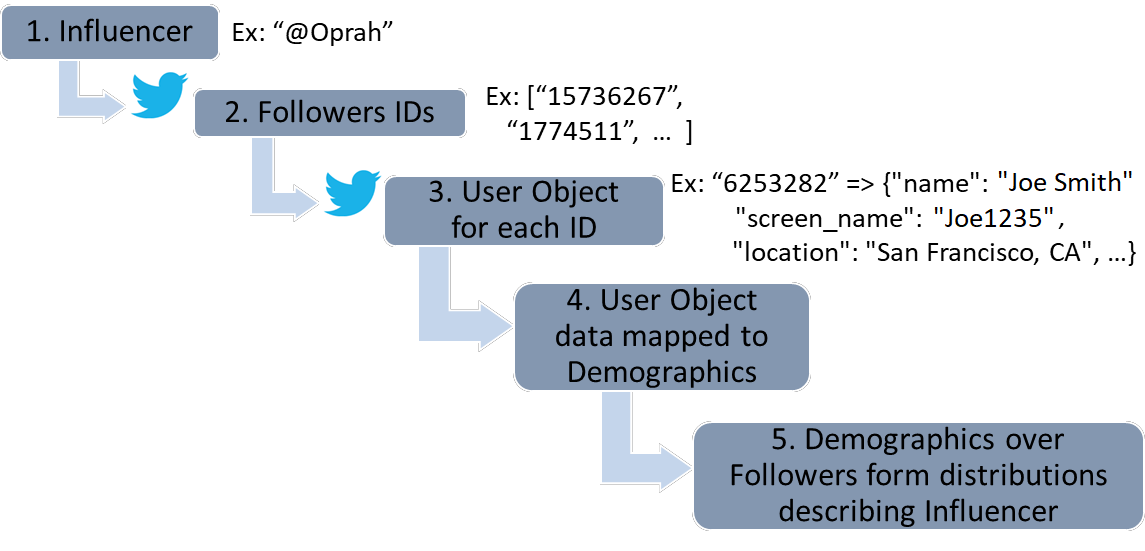
\includegraphics[width=5.4in]{Fig1}
\caption[Category 1 vs. Category 2 location frequency]{Category 1 are locations with a high accuracy where at least 75\% of users post messages with coordinates that are within 100 miles of coordinates geocoded from the self-reported location. Category 2 has low accuracy where less than 3.4\% of users match.}
\label{fig_ch2_1}
\end{figure}

\section{Classifier for Identifying Poor Geocoding}

Google's geocoder will attempt to geocode queries such as `my house' by matching to a business name. Such self-reported locations are common on Twitter due to the user being purposely ambiguous to preserve privacy. The classifier utilizes features, such as overlap between query and geocoder's associated address components, in order to make a prediction of whether Google's geocoder should be trusted.

\subsection{Features}

\begin{table}
\small
\renewcommand{\arraystretch}{1.2}
\caption{Google Geocoder Output}
\label{table_ch2_4}
\centering
\begin{tabular}{|c|c|}
\multicolumn{2}{c}{Additional Google Geocoder Output besides Coordinates}\\
\hline
\bfseries Output Type & \bfseries Description\\
\hline
address & Each component consists of the component type, short name, \\
components & and long name. Example types are country, ADM1 (state), \\
& ADM2 (county), locality (city), street number, route, \\
& neighborhood name, postal code, and others. \\
 \hline
formatted address&	Full address matched by Google, may not include all of \\
& the address components (for example county usually omitted). \\
 \hline
address & Describes what the address is associated with, example values: \\
type & point of interest, university, restaurant, and others. \\
\hline
\multicolumn{2}{c}{}\\
\multicolumn{2}{c}{Google Geocoder Output for query `New York, New York'}\\
\hline
\bfseries Output Type & \bfseries Output Value\\
\hline
coordinates & lat: 36.1023715, lng: -115.1745559\\
\hline
address & street\_number: 3790, route: South Las Vegas Boulevard\\
components & locality: Las Vegas, ADM2: Clark County, ADM1:\\
& Nevada, country: United States, postal\_code: 89109\\
\hline
formatted address& 3790 S Las Vegas Blvd, Las Vegas, NV 89109, USA\\
\hline
address type & casino, establishment, lodging, point\_of\_interest\\
\hline
\end{tabular}
\end{table}

\begin{table}
\small
\renewcommand{\arraystretch}{1.2}
\caption[Top 10 Most Frequent Address Type and Address Component]{Top 10 Most Frequent Address Type (Left) and Component (Right)}
\label{table_ch2_6}
\centering
\begin{tabular}{|c|c||c|c|}
\hline
\bfseries Address Type & \bfseries Ratio & \bfseries Address Component & \bfseries Ratio \\
\hline
political&0.6298&country&1\\
\hline
locality&0.566&administrative\_area\_level\_1&1\\
\hline
establishment&0.3101&locality&0.9639\\
\hline
point\_of\_interest&0.3068&administrative\_area\_level\_2&0.9481\\
\hline
store&0.0563&postal\_code&0.5652\\
\hline
food&0.0511&route&0.3348\\
\hline
neighborhood&0.04&street\_number&0.3027\\
\hline
restaurant&0.0395&administrative\_area\_level\_3&0.2005\\
\hline
university&0.0249&neighborhood&0.1827\\
\hline
route&0.0246&postal\_code\_suffix&0.1308\\
\hline
\end{tabular}
\end{table}

Table \ref{table_ch2_4} shows additional output, Google's geocoder produces, besides the latitude and longitude coordinates, and gives as an example, the output for query `New York, New York'. Notice that for the query, the street number in address components as well as the address types: (i) casino, (ii) establishment, (iii) lodging are indicative of an address that is a street level address (which could be used to assign a lower confidence for this prediction).

Across all of the locations in our dataset, there were a total of 73 unique address components and 116 unique address types. Table \ref{table_ch2_6} shows the top 10 address components and address types that account for the biggest ratio of all locations. The address types of store, food, restaurant should not represent a plausible location that most Twitter users will associate themselves with, but surprisingly over 5\% of locations in our dataset are some sort of a store (indicating potential errors). 

After looking at all address components, our expectation was that most Twitter users will report a location that is associated with: (i) political entity, (ii) zip, or (iii) university address type (as these are large enough to be reasonable locations to associate with). A location with one or more of these attributes is classified as a high-level location; otherwise, it is classified as low-level (street-level). 

\begin{figure*}[htp]
\centering
   \subfloat[Category 1]{\label{fig_ch2_2a}
      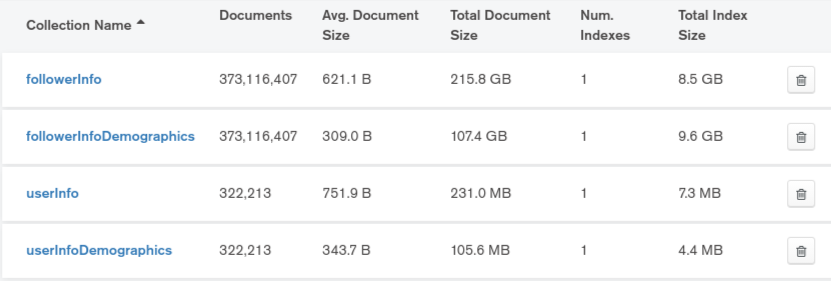
\includegraphics[width=.74\textwidth]{Fig2}}
\\
   %\hspace*{\fill}   % maximize separation between the subfigures
   \subfloat[Category 2]{\label{fig_ch2_2b}
      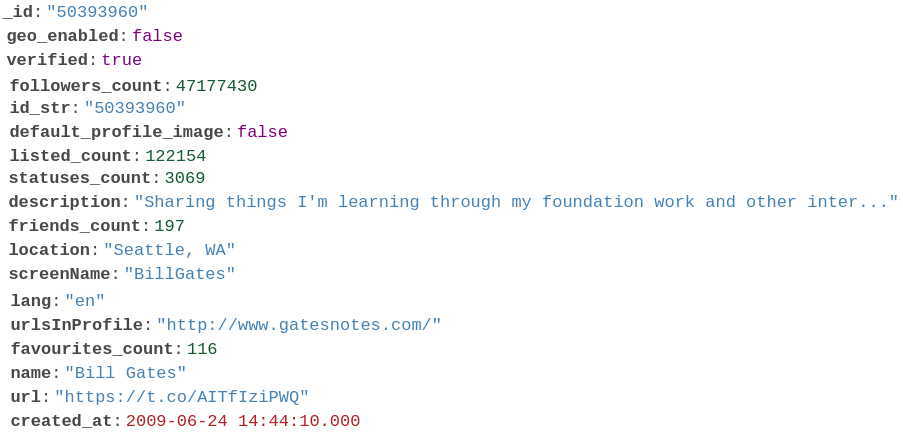
\includegraphics[width=.74\textwidth]{Fig3}}
   \caption[Category 1 vs. Category 2 ratio street-level]{\textbf{Top} -- Large ratio of Category 1 locations associated with a high-level address (as in city-level). \textbf{Bottom} -- Large ratio of Category 2 locations (impossible to geocode) are associated with low-level (as in street-level). The chart confirms that majority of properly geocoded locations are not at street-level.} \label{fig_ch2_2}
\end{figure*}

Fig. \ref{fig_ch2_2} (top) shows that the majority of category 1 locations get associated with a high-level location type. This is especially true as the minimum number of users that utilize location increases. For locations with number of users $\geq 100$, the high-level location type captures 99.6\% (843 out of 846) of category 1 locations. 

Conversely, Fig. \ref{fig_ch2_2} (bottom) shows inaccurately geocoded locations captured by category 2 are associated with low-level location type. The overall trend does not decrease, but the number of associated mistakes is small because the number of category 2 locations is small (only 43 locations used by at least 100 users). %$\geq 100$ per location the high-level location type captures 32.56\% (14 out of 43) of category 2 locations. 
Examples of locations that do get associated with a high-level location type: Midwest to Midwest WY, Nederland to Nederland CO, Nowhere to Nowhere OK, Moon to Moon PA, and others where a popular concept matches a city name. 

A number of additional features were proposed based on overlap between query and geocoder association. All of the features proposed are summarized below:

\begin{itemize}
\item F1: Political Entity = political address type without a street number address component. The political address type refers to recognized divisions of a physical territory; locality, neighborhood, colloquial area, sub-locality, and others.
\item F2: Zip = postal code address type
\item F3: University = university address type
\item F4: Text Overlap = returns percent character overlap between textual self-reported location and textual address associated by the geocoder.
\item F5: City/State exact = returns true if tokens from the query can be combined to match city and state address component exactly, false otherwise. 
\item F6: Populous City = for unique cities with a population over 50K, it is assumed that city name may be known to most human users such that the state need not be spelled out. Location matched to 2016 US census data using city and state that Google associates with the query string.
\end{itemize}

\subsection{Classifier}

Accurately geocoded locations (TRUE label) are those with $ACC@100$ $\geq$ 0.75 (category 1). Impossible to geocode locations (FALSE label) are those with $ACC@100$ $\leq$ 0.035 (category 2) (each self-reported location used by at least fifty users). The classifier utilizes the proposed features for predicting when Google's geocoder will perform poorly. 

For the classifier, we considered Naïve Bayes and Decision Tree (using gain ratio, information gain, and Chi-square interaction detector (CHAID)). Classifier trained using 5-fold-cross-validation utilizing the RapidMiner software package. Fig. \ref{fig_ch2_4} shows, the best performing classifier, Decision Tree using the CHAID criterion. 

\subsection{Performance}

Table \ref{table_ch2_7} compares the performance using three error measures proposed for locations that pass and fail classifier. Out of 131,925 self-reported locations in our dataset, 46,091 or 35\% were classified as low confidence (Google geocoder's output should not be trusted for these). Under 20\% of users with such locations are confirmed using message coordinates (illustrating that they do indeed have poor performance). In contrast, for those locations that pass the classifier, over 80\% of users are confirmed via message coordinates.   


\begin{figure}[!t]
\centering
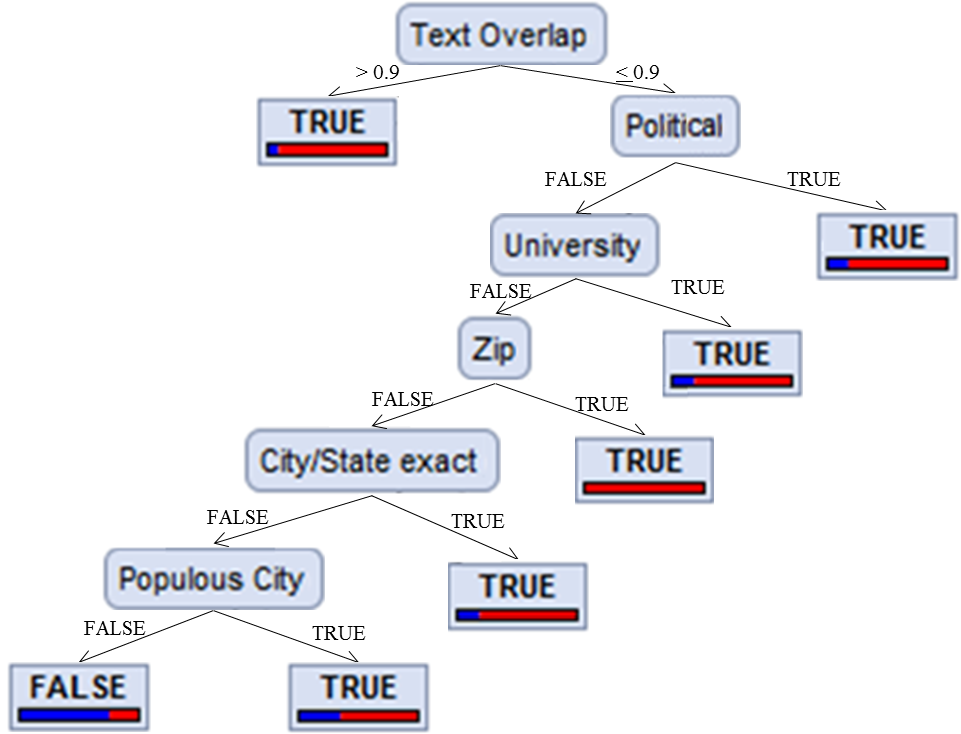
\includegraphics[width=3in]{Fig4}
\caption{Decision Tree Classifier for Identifying Geocoding Errors}
\label{fig_ch2_4}
\end{figure}

\begin{table}
\small
\renewcommand{\arraystretch}{1.2}
\caption{Geocoding Performance over Users}
\label{table_ch2_7}
\centering
\begin{tabular}{|c|c|c|c|}
\hline
\bfseries Location Set & \bfseries MeanED & \bfseries MedianED & \bfseries ACC@100\\
\hline
Fail Classifier&1705.12&879.45&0.1969\\
\hline
Pass Classifier&237.1&6.3&0.8027\\
\hline
\end{tabular}
\end{table}

The rules of the classifier illustrate that it is important to consider whether a location that is matched by the geocoder contains both the city and state as this is less ambiguous than a city name by itself. Google's geocoder is limited by the amount of API calls it can freely make daily and thus matching using a rule-based approach (using locations that contain a known city/state or city/country) is an option for a high precision/low recall solution.

\section{Conclusions}
The research has explored various types of geocoding errors and has established expected error rates for well and poorly geocoded locations in the context of Twitter. These measures were used to develop a classifier for whether the commercial off-the-shelf geocoder is performing as it should on Twitter data. In our dataset, close to 35\% of self-reported locations geocoded using Google resulted in a warning. Under 20\% of users with such locations were confirmed using message coordinates, illustrating that the Geocoder does exhibit a poor performance for these locations. In contrast, for those locations that pass the classifier, over 80\% of users are confirmed via message coordinates. In the next chapters, for those users whose location cannot be determined from textual self-reported location, other features will be described for inferring location.